\documentclass{beamer}

\usepackage[frenchb]{babel}
\usepackage[utf8]{inputenc}  
\usepackage[T1]{fontenc}
\usepackage[lined,ruled,boxed,linesnumbered]{algorithm2e}
\usepackage{amsmath,amsfonts,amsbsy,amssymb,mathabx,amsthm,bbm,bm} 
\usepackage{graphicx}
\usepackage{arydshln}
\usepackage{stmaryrd}

\usetheme{Warsaw}

\title{Codes LDPC}
\author{Banier Corentin et Karboul Maher}
\institute{Université de Bordeaux}
\date{18 Mai 2021}

\begin{document}
	\begin{frame}
        \titlepage
	\end{frame}

    \begin{frame}
        \frametitle{Introduction et présentation des objectifs}
        Dans ce travail, nous allons étudier, dans un premier temps, comment fabriquer des instances de code LDPC notamment avec le modèle de Mr.Gallager. 
        Puis, nous comprendrons comment décoder ces codes en effectuant un tas d'expériences. Et à la fin de ce projet, on essaiera "d'optimiser" ce dernier en 
        limitant le nombre d'équation à satisfaire par un mot de code erroné.
    \end{frame}

    \begin{frame}
        \frametitle{Définition d'un code LDPC}
        \textsc{\textbf{\underline{Définition :}}} Un code LDPC régulier est défini comme l'espace nul d'une matrice de contrôle de parité $H$, qui a les propriétés suivantes:
        \begin{enumerate}
            \item Chaque ligne à $p$ valeurs 1.
            \item Chaque colonne à $q$ valeurs 1.
            \item $p$ et $q$ ont des petites valeurs en comparaison avec la longueur du code et avec le nombre de ligne de la matrice $H$.
        \end{enumerate}
    \end{frame}

    \begin{frame}
        \frametitle{Réprésentation des codes LDPC}
        Les codes LDPC peuvent être représentés sous forme matricielle ou sous la forme d'un graphe biparti.
        \newline Par exemple, la matrice suivante:
        $$H=
        \begin{pmatrix}
            1 & 0 & 0 & 0 & 1 & 0 & 0 & 0 \\
            0 & 1 & 0 & 0 & 1 & 1 & 0 & 0 \\
            0 & 0 & 1 & 0 & 0 & 1 & 1 & 0 \\
            0 & 0 & 0 & 1 & 0 & 0 & 1 & 1 
        \end{pmatrix}
        \quad
        $$
        Peut être définie de la manière suivante:
        \begin{figure}[!h]
            \centering
            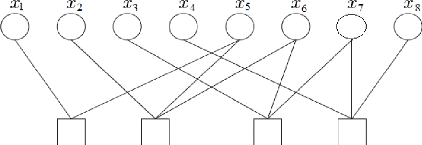
\includegraphics[scale=0.5]{Tanner2.png}  
            \caption{Graphe de Tanner associé à $H$}
            \label{fig:Tanner2}
        \end{figure}
    \end{frame}

    \begin{frame}
        \frametitle{Construction des codes LDPC}
        \framesubtitle{Robert Gray Gallager}
        \begin{columns}
            \begin{column}{5cm}
                \begin{figure}[!h]
                    \centering
                    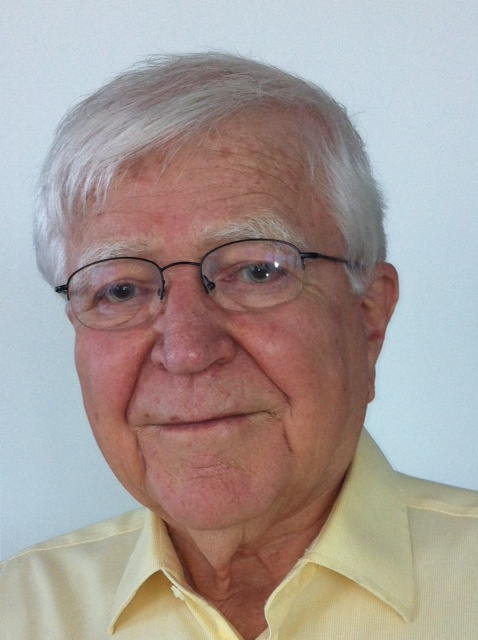
\includegraphics[scale=0.2]{Robert_Gallager.jpg} 
                    \caption{Mr. Robert Gray Gallager} 
                    \label{fig:gallager}
                \end{figure}
                Ingénieur Américain né en 1931.
            \end{column}
            
            \begin{column}{5cm}
                \begin{itemize}
                    \item Travaux sur le théorie de l'information.
                    \item Publication en 1963 de sa thèse sur les codes de contrôle de parité de basse densité (LDPC).
                    \item Rédacteur en chef adjoint sur le codage au sein de l’IEEE Transactions on Information Theory de 1963 à 1964.
                    \item Rédacteur associé pour les communications informatiques de 1977 à 1980.
                \end{itemize}
            \end{column}
            \end{columns}
    \end{frame}

    \begin{frame}
        \frametitle{Construction des codes LDPC}
        \framesubtitle{La construction de Gallager}
        Voici un exemple d'une matrice de Gallager:
        $$H=
        \begin{bmatrix}
            1 & 1 & 1 & 1 & 1 & 0 & 0 & 0 & 0 & 0 \\
            0 & 0 & 0 & 0 & 0 & 1 & 1 & 1 & 1 & 1 \\
            \hdashline
            1 & 0 & 1 & 0 & 0 & 1 & 0 & 1 & 0 & 1 \\
            0 & 1 & 0 & 1 & 1 & 0 & 1 & 0 & 1 & 0 \\
            \hdashline
            1 & 1 & 0 & 0 & 1 & 0 & 1 & 0 & 0 & 1 \\
            0 & 0 & 1 & 1 & 0 & 1 & 0 & 1 & 1 & 0 
        \end{bmatrix}
        \quad
        $$
    \end{frame}

    \begin{frame}
        \frametitle{Construction des codes LDPC}
        \framesubtitle{Construction utilisée pour nos tests}
        Pour nos expérimentations, nous avons créer une fonction qui nous produit une matrice de la forme suivante:
        \begin{equation*}
            H = \left[
            \begin{array}{cccccccccccccc}
                1&0&0&0&1&0&1&0&0&1&0&1&1&0 \\
                1&1&1&1&1&0&0&0&0&0&1&1&0&1 \\
                1&1&0&0&0&1&0&1&0&0&0&0&0&0 \\
                0&0&1&0&0&0&1&1&1&0&1&0&1&0 \\
                0&1&0&0&1&1&0&0&1&0&0&0&1&1 \\
                0&0&1&1&0&1&1&0&0&1&0&1&0&0 \\
                0&0&0&1&0&0&0&1&1&1&1&0&0&1 
            \end{array}
            \right]
        \end{equation*}
    \end{frame}

    \begin{frame}
        \frametitle{Algorithme de décodage}
        \begin{figure}[!h]
            \centering
            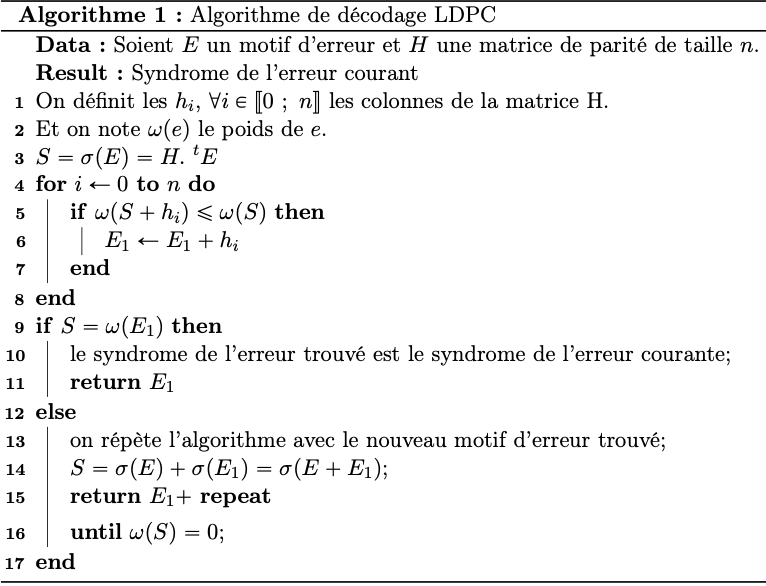
\includegraphics[scale=0.65]{algo.png}  
            \label{fig:algo}
        \end{figure}
    \end{frame}

    \begin{frame}
        \frametitle{Expérimentations}
        Modification de la ligne 5 de l'algorithme précédant: 
        \begin{center}
            $\omega(S + h_{i}) \le \omega(S)$
        \end{center}
        \vspace{0.4cm}
        On essaie d'exclure les positions parasites:
        $\omega(S + h_{i}) \le \omega(S) - a$, pour un entier $a$ fixé.
    \end{frame}

    \begin{frame}
        \frametitle{Expérimentations ; n=1000}
        \begin{figure}[h!]
            \centering
            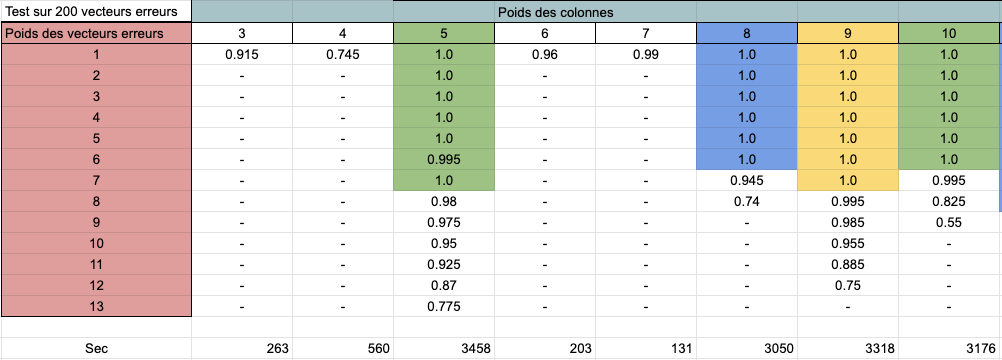
\includegraphics[scale=0.5]{res1000_n1.png}
            \label{fig:res1}
        \end{figure}
        \begin{figure}[h!]
            \centering
            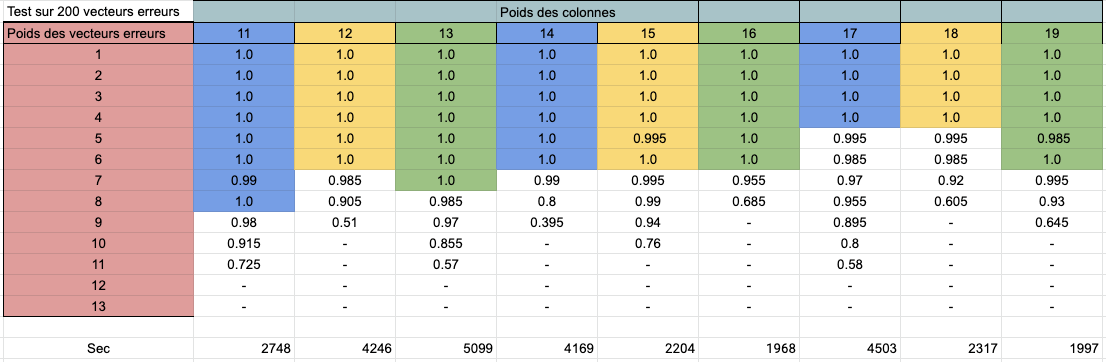
\includegraphics[scale=0.5]{res1000_n2.png}
            \label{fig:res2}
            \caption{Probabilité de décodage sur 200 vecteurs erreurs d'un certain poids en fonction du poids des colonnes d'une matrice de code LDPC}
        \end{figure}
    \end{frame}

    \begin{frame}
        \frametitle{Expérimentations ; n=1000}
        \begin{figure}[h!]
            \centering
            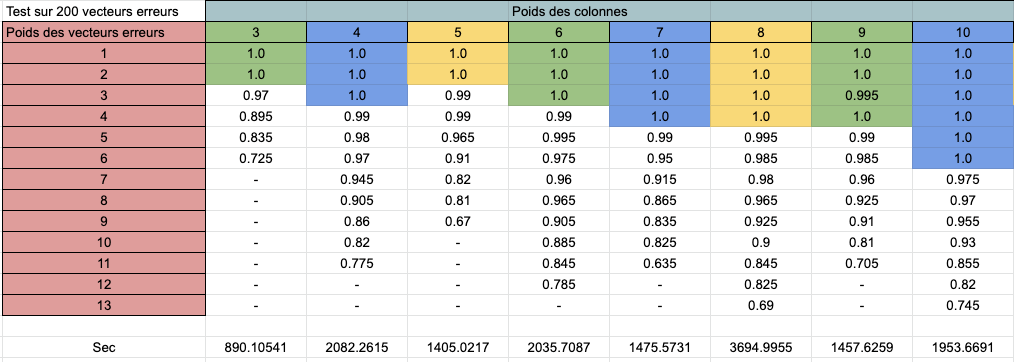
\includegraphics[scale=0.5]{res1000_opti1.png}
            \label{fig:res3}
        \end{figure}
        \begin{figure}[h!]
            \centering
            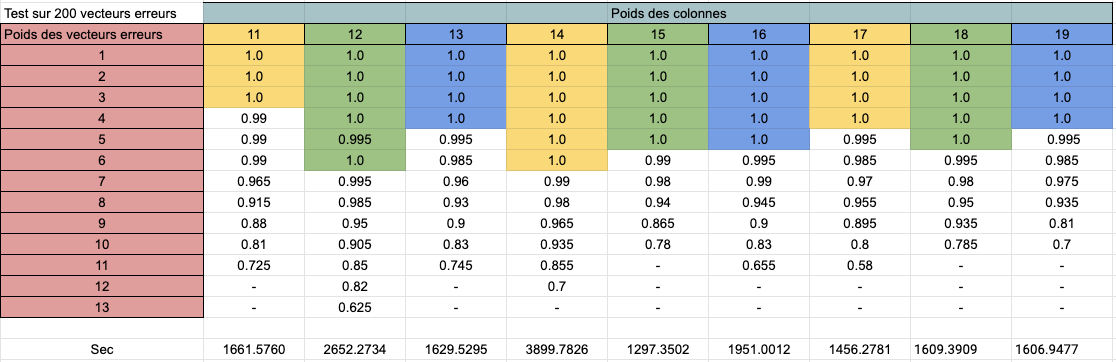
\includegraphics[scale=0.5]{res1000_opti2.png}
            \label{fig:res4}
            \caption{Probabilité de décodage sur 200 vecteurs erreurs d'un certain poids en fonction du poids des colonnes d'une matrice de code LDPC}
        \end{figure}
    \end{frame}

    \begin{frame}
        \frametitle{Expérimentations ; n=2000}
        \begin{figure}[h!]
            \centering
            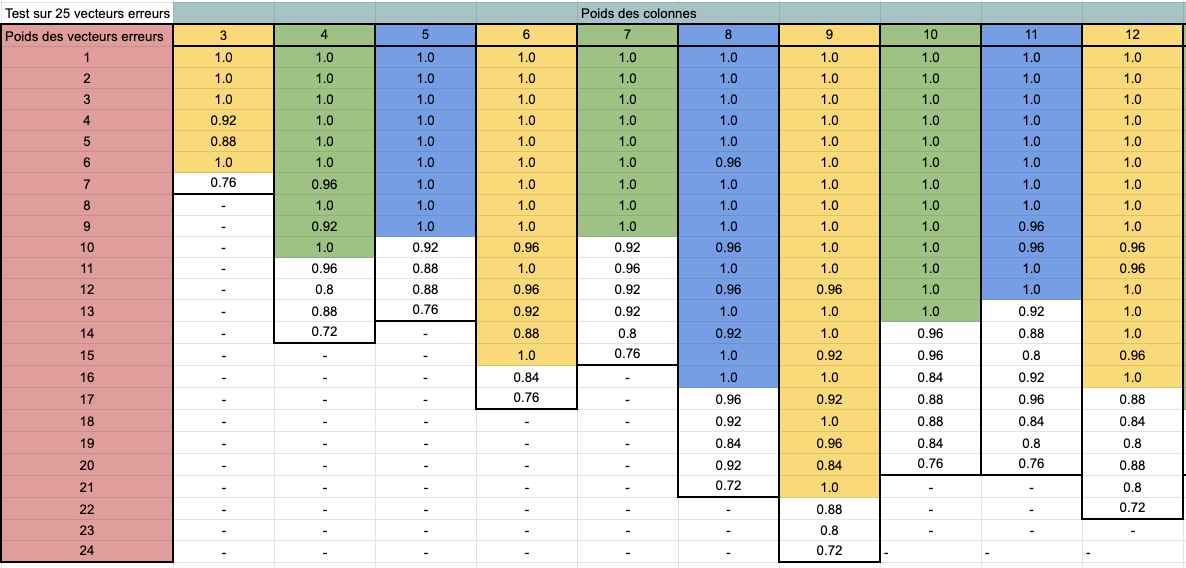
\includegraphics[scale=0.35]{res2000_1.png}
            \label{fig:res5}
        \end{figure}
        \begin{figure}[h!]
            \centering
            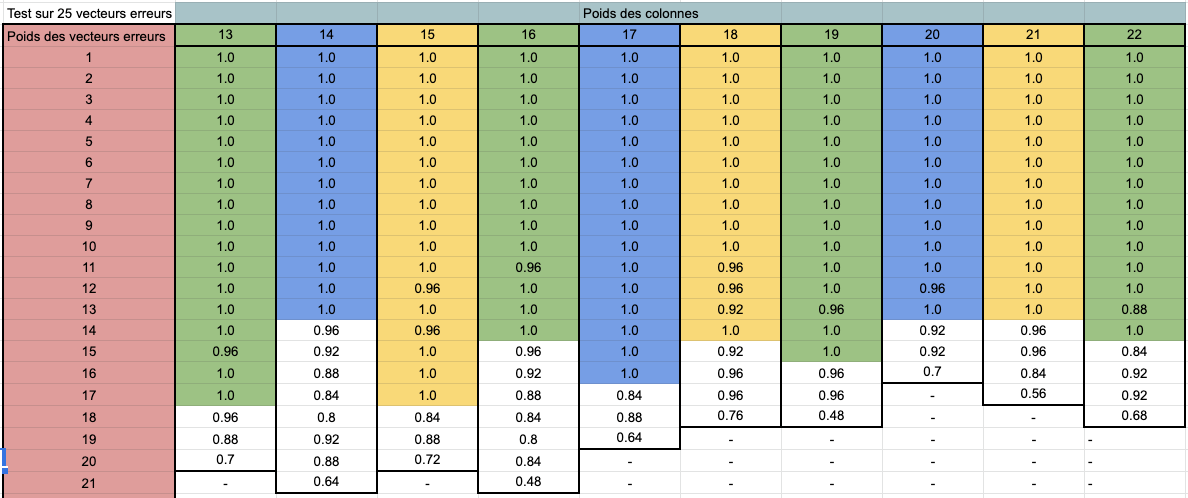
\includegraphics[scale=0.35]{res2000_2.png}
            \label{fig:res6}
            \caption{Probabilité de décodage sur 25 vecteurs erreurs d'un certain poids en fonction du poids des colonnes d'une matrice de code LDPC}
        \end{figure}
    \end{frame}

    \begin{frame}
        \frametitle{Conclusion}
        \begin{enumerate}
            \item Plus la taille des matrices augmente, plus l'algorithme de décodage fonctionne bien.
            \item La suppressions des positions parasites améliore la qualité des résultats mais on ne décode pas forcément plus.
            \item Une diminution exagérée du poids du syndrome entraine un oubli de certaine position érronée.
        \end{enumerate}
        \vspace{1cm}
        Nous adressons nos remerciements à Mr. Zémor Gilles de nous avoir guider dans la réalisation et l'implémentation de ce projet.

    \end{frame}

\end{document}